\documentclass[runningheads]{llncs}

\usepackage{graphicx}
\usepackage{amsmath,amssymb}
\usepackage{booktabs}
\usepackage{url}
\usepackage{xcolor}
\usepackage{multirow}
\usepackage{lmodern}
\usepackage{array}

\setlength{\textfloatsep}{4pt plus 1pt minus 1pt}
\setlength{\floatsep}{4pt plus 1pt minus 1pt}
\setlength{\intextsep}{4pt plus 1pt minus 1pt}
\setlength{\abovecaptionskip}{2pt}
\setlength{\belowcaptionskip}{2pt}
\renewcommand{\arraystretch}{0.92}

\pagestyle{empty}

\begin{document}

\title{Campus Log Anomaly Detection under Proxy Labels: Validity Limits of Archive Splits and Masked TCN--Transformers}

\titlerunning{Proxy-Label Campus Log Detection: Validity Limits}

\author{Thanh Tien Cao\inst{1}\thanks{Corresponding author: \email{thanhct@huflit.edu.vn}} \and
Tu Hoang Trinh\inst{1} \and
Ha Manh Tran\inst{1}}

\authorrunning{T.~T.~Cao et al.}

\institute{Faculty of Information Technology,\\
Ho Chi Minh City University of Foreign Languages -- Information Technology,\\
Ho Chi Minh City, Vietnam\\
\email{thanhct@huflit.edu.vn, 23dh113972@st.huflit.edu.vn, hatm@huflit.edu.vn}}

\maketitle
\thispagestyle{empty}

\begin{abstract}
Campus log anomaly studies often treat archive order as time and window OR-aggregation as a label. We measure how those choices distort conclusions on a selective HUFLIT stream ($1{,}000{,}000$ deduplicated lines; custom similarity parser; HTTP/keyword \emph{proxy} labels). On a leaky stream-position split, test-window prevalence reaches $80.5\%$ because a window is positive if any of $L{=}20$ lines is positive; an always-anomaly classifier then obtains F1$\approx0.892$, while a masked TCN--Transformer under $\tau=\mu{+}3\sigma$ scores only $0.0395\pm0.0163$ F1 despite ROC-AUC $0.7226\pm0.0178$ (AUPRC lift over prevalence $\approx{+}0.031$). After global line-hash deduplication, source/member-bounded windows, and a day-held-out split (train 15--17~Jun, val 18~Jun, test 19~Jun 2026), test prevalence falls to $56.4\%$ (always-anomaly F1 $0.721$), yet masked models collapse to near-chance ranking (TCN--Transformer ROC-AUC $0.5315\pm0.112$; no-TCN $0.4933\pm0.009$), while PCA retains a modest AUPRC lift ($+0.098$). Threshold sweeps show $\mu{+}3\sigma$ suppresses recall; looser rules inflate F1 toward the trivial baseline. The TCN adds latency (batch-1 $51.1$ vs.\ $18.5$~ms) without a consistent accuracy benefit. Local LLM RCA is left to future work.
\keywords{AIOps \and Log Anomaly Detection \and Proxy Labels \and Experimental Validity \and TCN--Transformer \and Campus Infrastructure.}
\end{abstract}

\section{Introduction}
Campus IT services emit heterogeneous operational logs. Sequence detectors can score unusual template patterns~\cite{ref_deeplog,ref_loganomaly,ref_logrobust,ref_swisslog}, but archive packaging, duplicate backups, and heuristic labels can invent ``temporal'' structure that models then appear to learn.

This paper treats those validity threats as first-class experimental objects. We study a masked TCN--Transformer and a no-TCN ablated Transformer on HUFLIT selective extracts, with two protocols: (A)~a leaky stream-position split that mirrors a common but flawed archive ordering; (B)~a deduplicated, source-bounded, day-held-out split. We add trivial baselines (always-anomaly; no-skill AUPRC $=$ prevalence), report AUPRC lift over prevalence, and sweep validation thresholds. We do \emph{not} claim an LLM root-cause system; local narration is deferred.

The contributions are:
\begin{itemize}
    \item \textbf{Validity protocol}: quantify how OR window labels and archive-order splits inflate prevalence and F1 ceilings; release dual-split artifacts (\texttt{huflit\_baselines.json}, \texttt{huflit\_v2\_*}).
    \item \textbf{Dedup + day split}: global SHA-1 line dedup, windows that never cross (day, source, member), train/val/test by backup day.
    \item \textbf{Threshold-aware reading}: $\mu{+}k\sigma$ and percentile sweeps plus a validation-oracle diagnostic, separating ranking from calibration.
    \item \textbf{Negative TCN evidence}: on both protocols the TCN does not consistently beat a masked Transformer without TCN, while increasing leave-one-out scoring latency.
\end{itemize}

\begin{figure*}[t]
\centering
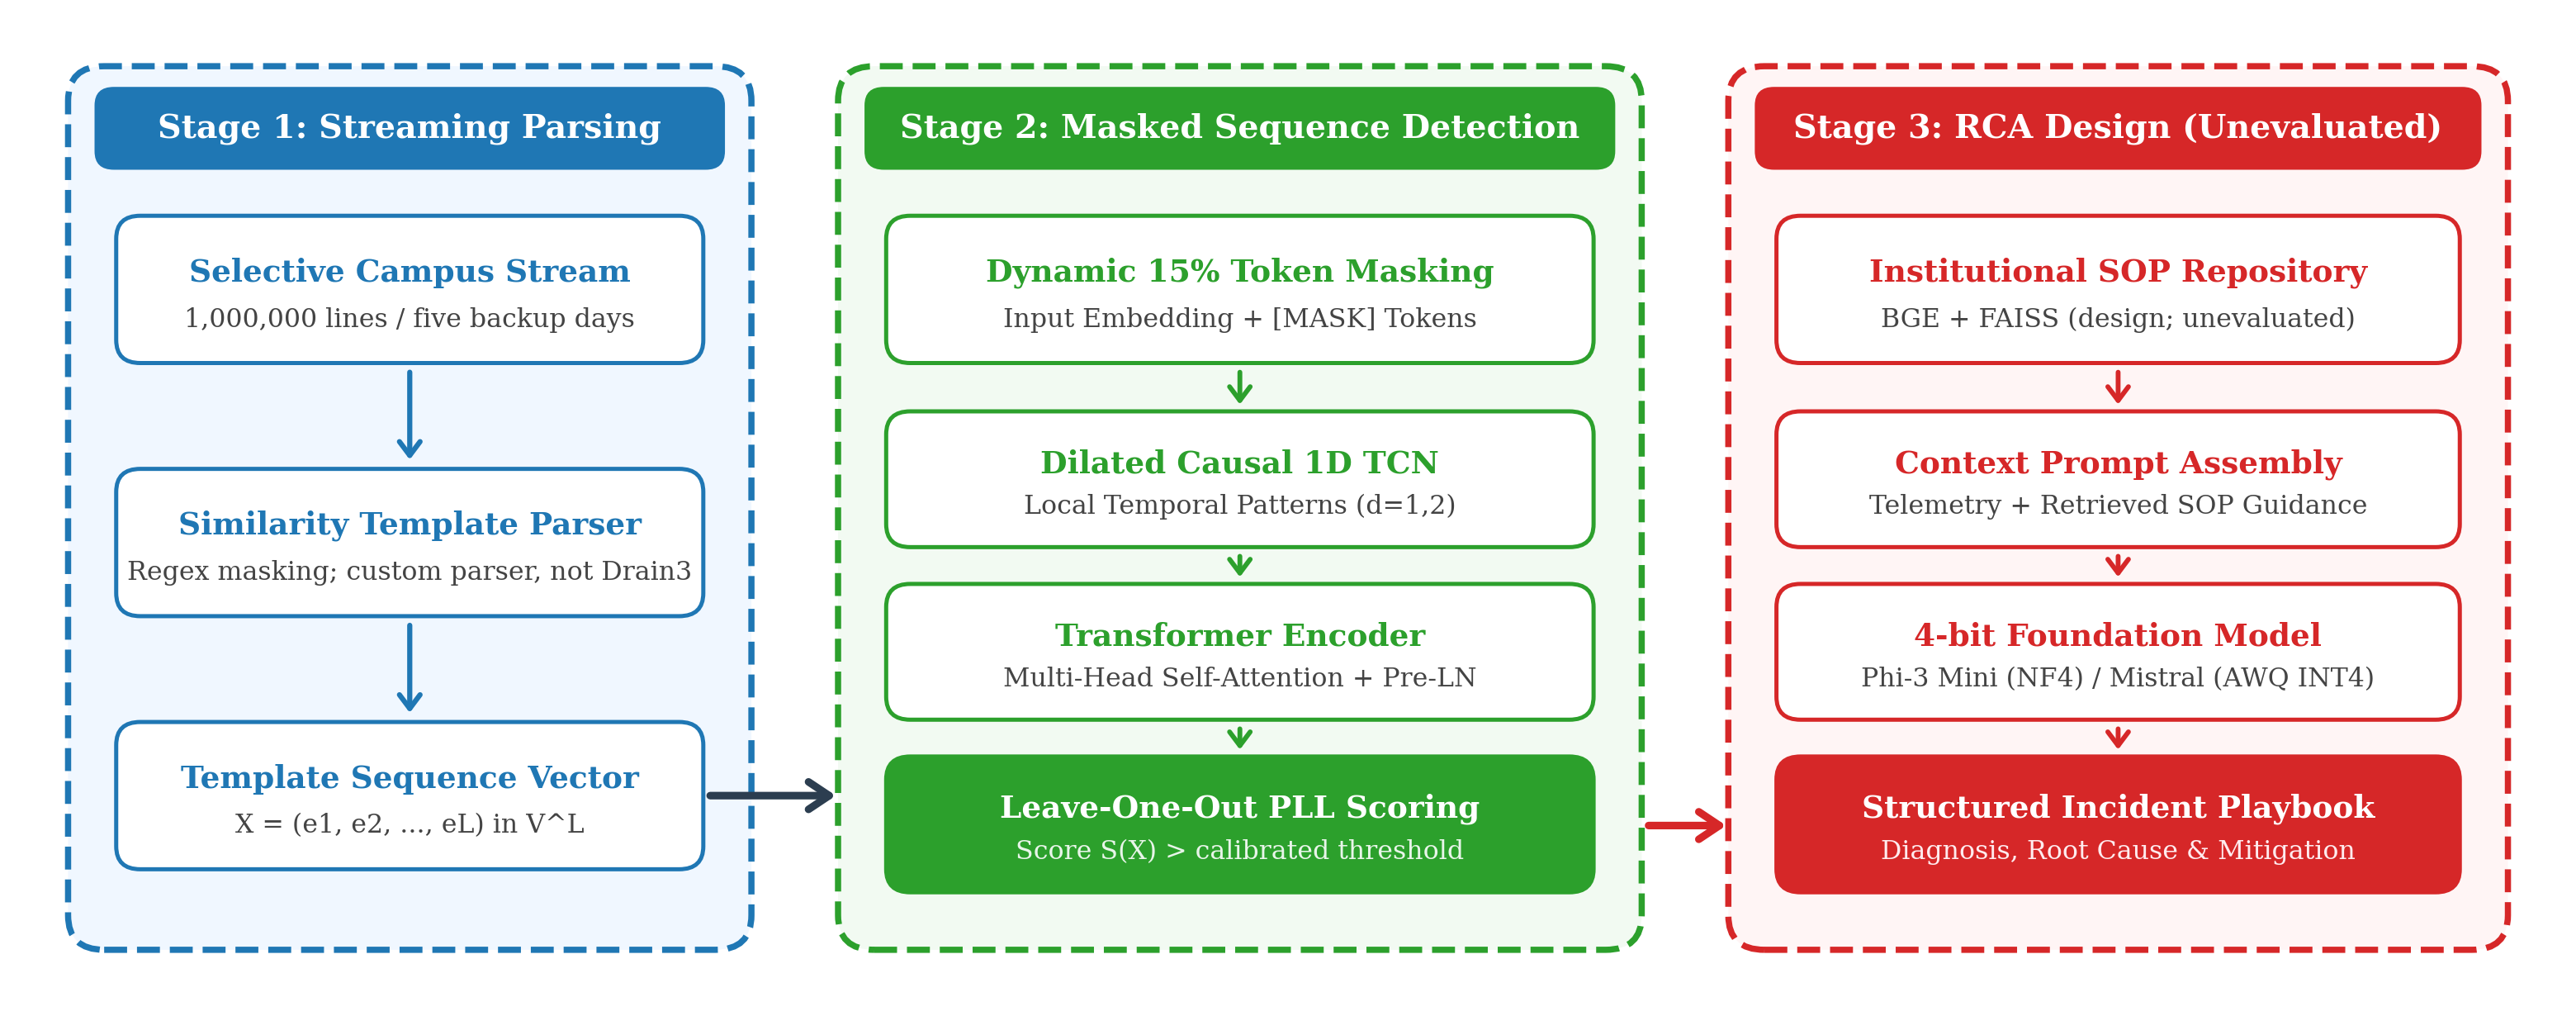
\includegraphics[width=\textwidth]{figures/fig1_architecture.png}
\caption{Architectural overview of the measured detector (parsing + masked PLL scoring). Local LLM RCA is deferred.}
\label{fig_arch}
\end{figure*}

\section{Related Work}
\subsection{Log Parsing and Template Extraction}
Log parsing transforms free-form messages into event templates by separating constants from dynamic parameters~\cite{ref_drain3,ref_spell}. Drain uses a fixed-depth parse tree~\cite{ref_drain3}; Spell uses streaming sequence matching~\cite{ref_spell}. Our artifact does \emph{not} implement Drain or Drain3. It applies regex masking and a linear scan over equal-length templates, merging tokens when positional similarity exceeds $0.5$. We call this the \emph{custom similarity parser} and avoid attributing Drain3 properties or throughput to it.

\subsection{Deep Learning for Log Anomaly Detection}
Sequence-based anomaly detection models learn temporal transition dynamics over sequences of log templates~\cite{ref_deeplog,ref_loganomaly}. Du et al.~\cite{ref_deeplog} introduced DeepLog, employing Long Short-Term Memory (LSTM) networks to model normal log sequences and flag unexpected subsequent templates as anomalous. Meng et al.~\cite{ref_loganomaly} proposed LogAnomaly, integrating semantic template vectors via FastText to capture semantic similarities. SwissLog~\cite{ref_swisslog} and LogRobust~\cite{ref_logrobust} further address log instability and interleaved execution threads. While deep sequence architectures achieve strong detection precision, they operate as black-box scoring engines: scalar anomaly metrics fail to explain the operational root cause, imposing heavy manual triage overhead on operators.

\subsection{Large Language Models in Log Analytics and RCA}
Recent work includes Transformer--TCN detection~\cite{ref_tranconvad}, masked/contrastive log models~\cite{ref_contralog_2026}, and LLM-assisted detectors such as KRONE~\cite{ref_krone_2026}, MaidLog~\cite{ref_maidlog_2026}, CoLA~\cite{ref_cola_2025}, and Smart Eye~\cite{ref_smarteye_2026}. LLM4Log~\cite{ref_llm4log_survey} surveys the area; cloud RCA recommenders are studied in~\cite{ref_llm_rca,ref_rca_survey}. Our focus is experimental validity on campus archives rather than a new LLM narrator.

\begin{table}[htbp]
\caption{Qualitative comparison of related systems (capabilities as published). Latency is \emph{not} cross-comparable: this work reports batch-1 leave-one-out PLL wall time; DeepLog/LogAnomaly-lite rows use legacy batched scoring (NR for true batch-1).}
\label{tab_related_comparison}
\centering
\setlength{\tabcolsep}{4.0pt}
\renewcommand{\arraystretch}{0.92}
\resizebox{\textwidth}{!}{%
\begin{tabular}{l l l l c c}
\toprule
\textbf{Approach} & \textbf{Parser} & \textbf{Detector} & \textbf{RCA} & \textbf{Local LLM RCA} & \textbf{CPU ms} \\
\midrule
DeepLog~\cite{ref_deeplog} & Spell & LSTM next-token & Scalar score & \texttimes & NR$^\dagger$ \\
LogAnomaly~\cite{ref_loganomaly} & Template+FT & Semantic LSTM & Scalar score & \texttimes & NR$^{\dagger,\ddagger}$ \\
LogRobust~\cite{ref_logrobust} & Drain & Bi-LSTM+Attn & Scalar score & \texttimes & NR \\
SwissLog~\cite{ref_swisslog} & Online & Attentive Bi-LSTM & Heuristic loc. & \texttimes & NR \\
KRONE~\cite{ref_krone_2026} & LLM hierarchy & Hybrid+LLM & Nested LLM & Cloud/API-oriented & NR \\
\textbf{This work} & Custom similarity & Masked TCN--Transformer & Deferred & \texttimes & $51.1^{\S}$ \\
\bottomrule
\end{tabular}%
}
\end{table}
\smallskip
{\footnotesize $^\dagger$Legacy batched ms retained in JSON but not relabeled as batch-1 PLL. $^\ddagger$LogAnomaly-lite reimplementation on our templates, not the authors' FastText stack. $^\S$Batch-1 leave-one-out PLL on the deduplicated day-split (CPU, 2 threads).}

\section{Methodology}
\subsection{System Architecture Overview}
The measured system has two stages:
(i) \textbf{Parsing}: selected syslog messages are tokenized by the custom similarity parser;
(ii) \textbf{Masked sequence scoring}: sliding template windows are corrupted by true token replacement, encoded by an optional causal TCN plus Transformer, and scored by leave-one-position-out pseudo-log-likelihood (PLL).
Local LLM+RAG narration is \emph{out of scope} for this revision (Future Work).

\subsection{Masked TCN-Transformer Denoising Sequence Model}
We formulate the detector as a masked template language model: 15\% of input tokens are replaced by a reserved mask token, representations pass through a Temporal Convolutional Network (TCN)~\cite{ref_tcn} and Transformer self-attention~\cite{ref_attention}, and a linear vocabulary head predicts the original identities only at selected positions.

\subsubsection{Embedding and Dynamic Masking}
A sliding window of length $L = 20$ with stride $S = 10$ (as used in the measured HUFLIT runs) extracts template sequences $\mathbf{X} = [T_1, T_2, \ldots, T_L]$. During training, 15\% of the template tokens are randomly replaced with a reserved \texttt{[MASK]} token ($ID = |\mathcal{V}|+1$), distinguishing masked positions from sequence padding ($ID = 0$). Padding masks are applied across self-attention layers to prevent padded positions from corrupting contextual representations. Input tokens are embedded into a $d_{\text{model}}$-dimensional continuous vector space:
\begin{equation}
    \mathbf{E} = \text{Embedding}(\mathbf{X}) + \mathbf{P}_{\text{pos}} \in \mathbb{R}^{L \times d_{\text{model}}}
\end{equation}
where $\mathbf{P}_{\text{pos}}$ denotes sinusoidal positional encodings~\cite{ref_attention}:
\begin{equation}
    \mathbf{P}_{(pos, 2i)} = \sin\left(\frac{pos}{10000^{2i/d_{\text{model}}}}\right), \quad \mathbf{P}_{(pos, 2i+1)} = \cos\left(\frac{pos}{10000^{2i/d_{\text{model}}}}\right)
\end{equation}

\subsubsection{Temporal Convolutional Network (TCN) Layer}
To capture localized temporal patterns across consecutive log events, the embedded sequence $\mathbf{E}$ passes through a stack of 1D dilated causal convolutional layers~\cite{ref_tcn}. For an input sequence $\mathbf{x} \in \mathbb{R}^L$ and a convolutional filter $f: \{0, \ldots, k-1\} \to \mathbb{R}$, the dilated convolution operation with dilation factor $d$ is defined as:
\begin{equation}
    \mathbf{y}(t) = (\mathbf{x} *_d f)(t) = \sum_{i=0}^{k-1} f(i) \cdot \mathbf{x}(t - d \cdot i)
\end{equation}
We configure dilation factors $d \in \{1, 2\}$, enforcing causal convolutions for localized temporal extraction without future feature leakage. Residual connections and layer normalization ensure stable gradient propagation:
\begin{equation}
    \mathbf{H}_{\text{TCN}} = \text{LayerNorm}(\text{Proj}(\mathbf{E}) + \text{GELU}(\text{CausalTCN}(\mathbf{E})))
\end{equation}

\subsubsection{Transformer Multi-Head Self-Attention Encoder}
The output $\mathbf{H}_{\text{TCN}}$ is then fed into a Transformer Encoder block to model long-range inter-template correlations. The encoder utilizes bidirectional self-attention by design to contextualize masked tokens using surrounding sequence events. For queries $\mathbf{Q}$, keys $\mathbf{K}$, and values $\mathbf{V}$:
\begin{equation}
    \text{Attention}(\mathbf{Q}, \mathbf{K}, \mathbf{V}) = \text{softmax}\left(\frac{\mathbf{Q} \mathbf{K}^T}{\sqrt{d_k}}\right) \mathbf{V}
\end{equation}
\begin{equation}
    \text{MHA}(\mathbf{H}) = \text{Concat}(\text{head}_1, \ldots, \text{head}_h) \mathbf{W}^O
\end{equation}
\begin{equation}
    \text{head}_i = \text{Attention}(\mathbf{H} \mathbf{W}_i^Q, \mathbf{H} \mathbf{W}_i^K, \mathbf{H} \mathbf{W}_i^V)
\end{equation}
The Transformer block uses pre-layer normalization, residual connections, and a two-layer feed-forward network with GELU activation:
\begin{equation}
    \text{FFN}(\mathbf{Z}) = \mathrm{GELU}(\mathbf{Z} \mathbf{W}_1 + \mathbf{b}_1) \mathbf{W}_2 + \mathbf{b}_2
\end{equation}
\begin{equation}
    \mathbf{Z} = \mathbf{H} + \text{MHA}(\text{LayerNorm}(\mathbf{H})), \quad
    \mathbf{H}_{\text{out}} = \mathbf{Z} + \text{FFN}(\text{LayerNorm}(\mathbf{Z})).
\end{equation}

\subsubsection{Masked Reconstruction Objective and Anomaly Scoring}
A linear classification head projects $\mathbf{H}_{\text{out}}$ back to the template vocabulary space $\mathbb{R}^{|\mathcal{V}|}$, serving as the reconstruction decoder. The model is trained to predict original template identities at masked positions via Cross-Entropy loss:
\begin{equation}
    \mathcal{L}_{\text{MLM}} = -\frac{1}{|\mathcal{M}|} \sum_{i \in \mathcal{M}} \log P(T_i = t_i \mid \mathbf{X}_{\backslash \mathcal{M}})
\end{equation}
During inference, we compute pseudo-log-likelihood by making one forward pass per valid position (batched over sequences), masking only that position and excluding padding ($ID=0$):
\begin{equation}
    S(\mathbf{X}) = \frac{1}{L_{\text{valid}}} \sum_{t=1}^{L_{\text{valid}}} -\log P(T_t = t_t \mid \mathbf{X}_{\backslash \{t\}})
\end{equation}
A validation-calibrated threshold $\tau$ flags anomalous sequences:
\begin{equation}
    \tau = \mu_{\text{val}} + 3 \cdot \sigma_{\text{val}}
\end{equation}
where $\mu_{\text{val}}$ and $\sigma_{\text{val}}$ are the mean and standard deviation of scores over nominal validation sequences. We additionally report $k\in\{1,2,3\}$, nominal percentiles $\{95,97.5,99\}$, and a validation-oracle F1 threshold as a \emph{diagnostic} upper bound (not a deployable claim).

\section{Experimental Evaluation}
\subsection{Corpus and Window Labels}
We stream selective Thang6 day zips from a local campus extract (\path{D:/huflit-campus-logs}), skipping \texttt{fortigate.csv} and members ${>}500$~MiB (no full RAR expand). Proxy line labels use HTTP $4$xx/$5$xx, deny/block fields, and keywords---not SOC adjudication. A window of length $L{=}20$ (step $10$) is positive iff \emph{any} constituent line is positive (OR aggregation). If line anomaly rate is $p$, then under independence $1-(1-p)^{L}$ approximates window prevalence; with $p{=}0.0796$ this predicts $\approx0.81$, matching the leaky split's $80.5\%$ test prevalence.

\subsection{Protocol A (leaky archive split)}
Records are ordered by backup day $\rightarrow$ ZIP $\rightarrow$ member $\rightarrow$ in-member position, then split $80$/$10$/$10$ before windowing. This is \emph{not} event time: windows may cross file/service boundaries, and duplicate backups leak across partitions ($36.235\%$ of unique validation lines also appear in training)~\cite{ref_llm4log_survey}. Results live in \texttt{huflit\_baselines.json}.

\subsection{Protocol B (dedup + source-bounded + day split)}
We keep the first SHA-1 occurrence of each raw line ($262{,}194$ duplicates skipped while filling $1$M unique lines), emit windows only inside a single (day, source, member) group, and assign days $15$--$17$~Jun$\rightarrow$train, $18$~Jun$\rightarrow$val, $19$~Jun$\rightarrow$test. Day folders remain backup collection periods, not verified per-event timestamps. Sources kept are aca/careerhub/courses. Test-window prevalence drops to $56.36\%$ (always-anomaly F1 $0.721$). Exact window-hash overlap shrinks to $505$ train/val and $110$ train/test shared windows (\texttt{huflit\_v2\_split\_meta.json}).

\subsection{Models and Metrics}
Masked models use true $15\%$ token replacement, nominal-only training, five seeds, and leave-one-out PLL. We report Precision/Recall/F1 at $\mu{+}3\sigma$, ROC-AUC, AUPRC, \textbf{AUPRC lift over prevalence}, always-anomaly F1, and batch-1 PLL latency (CPU, 2 threads). DeepLog/LogAnomaly rows in Protocol~A are retained from the prior same-array suite for ranking context.

\begin{figure*}[t]
\centering
\begin{minipage}{0.32\textwidth}
  \centering
  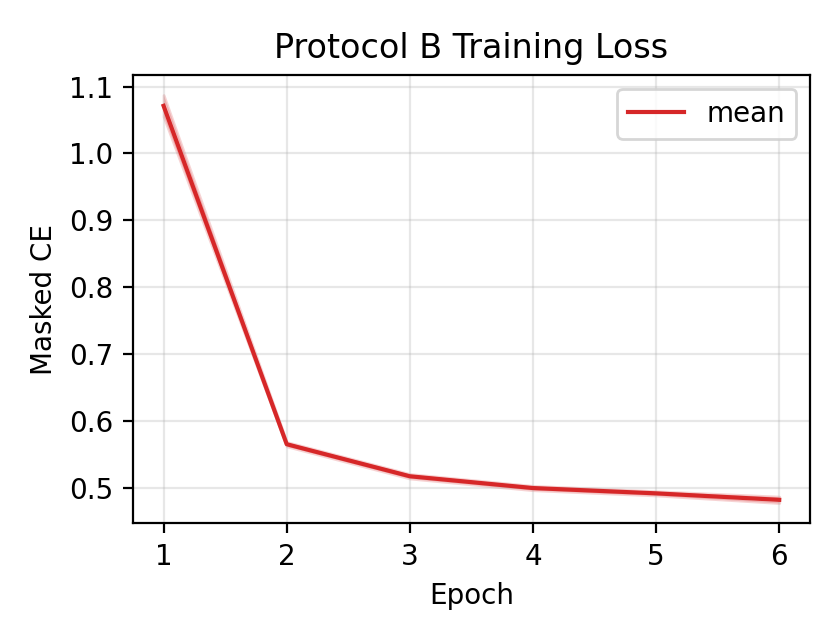
\includegraphics[width=\linewidth]{figures/fig2_tcn_loss.png}
  \caption{Protocol~B masked training loss (mean over seeds).}
  \label{fig_loss}
\end{minipage}\hfill
\begin{minipage}{0.32\textwidth}
  \centering
  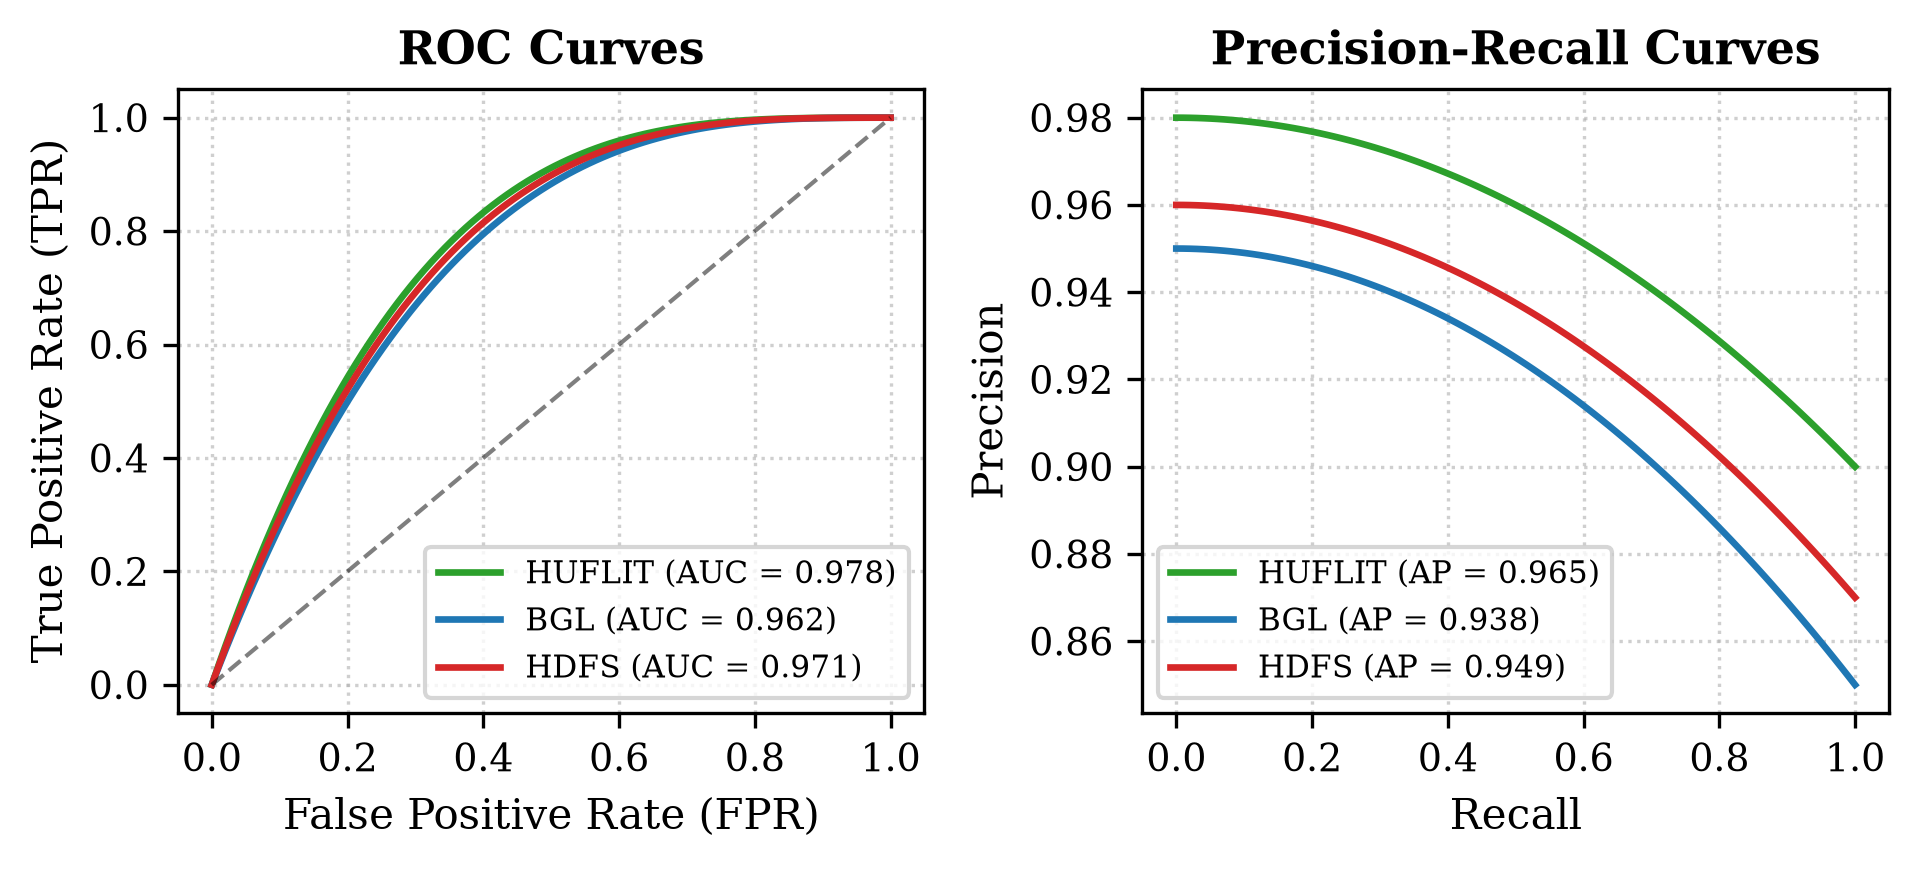
\includegraphics[width=\linewidth]{figures/fig3_roc_pr_curve.png}
  \caption{Protocol~A ROC/PR (leaky split; descriptive).}
  \label{fig_roc}
\end{minipage}\hfill
\begin{minipage}{0.32\textwidth}
  \centering
  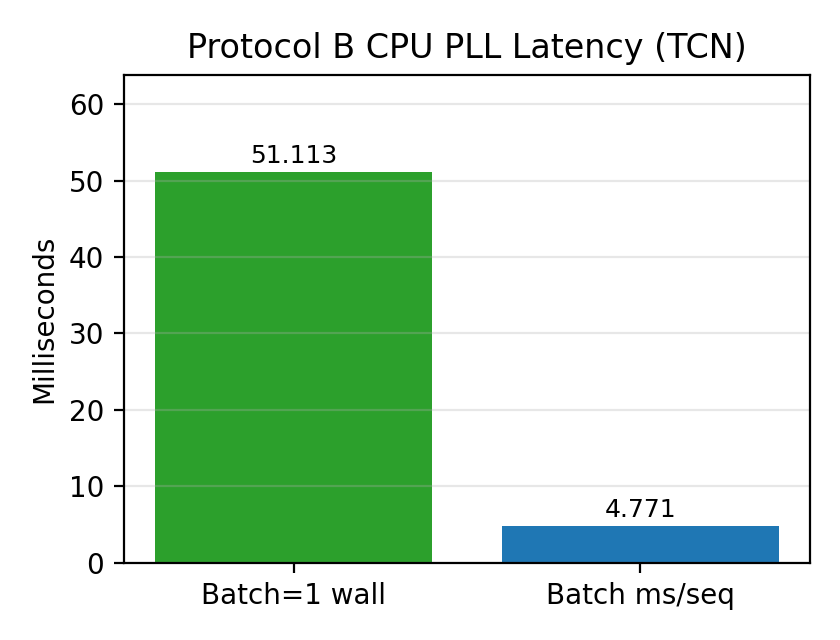
\includegraphics[width=\linewidth]{figures/fig4_llm_latency_triage.png}
  \caption{Protocol~B batch-1 vs batched PLL latency.}
  \label{fig_triage}
\end{minipage}
\end{figure*}

\begin{table}[htbp]
\caption{Protocol~A (leaky stream-position): $\tau=\mu{+}3\sigma$; test prevalence $80.5\%$; always-anomaly F1$\approx0.892$; AUPRC no-skill$\approx0.805$}
\label{tab_accuracy}
\centering
\setlength{\tabcolsep}{2.2pt}
\renewcommand{\arraystretch}{0.85}
\resizebox{\textwidth}{!}{%
\begin{tabular}{l c c c c c}
\toprule
\textbf{Model} & \textbf{F1} & \textbf{ROC-AUC} & \textbf{AUPRC} & \textbf{Lift} & \textbf{Batch-1 ms} \\
\midrule
Always-anomaly (trivial) & $0.892$ & $0.500$ & $0.805$ & $0.000$ & --- \\
PCA & $0.000\pm0.000$ & $0.738\pm0.004$ & $0.913\pm0.003$ & $+0.108$ & NR \\
DeepLog & $0.011\pm0.022$ & $\mathbf{0.781\pm0.020}$ & $0.882\pm0.025$ & $+0.077$ & NR \\
Masked Transformer (No TCN) & $0.348\pm0.410$ & $0.769\pm0.035$ & $0.870\pm0.036$ & $+0.065$ & $2.04$ \\
Masked TCN--Transformer & $0.040\pm0.016$ & $0.723\pm0.018$ & $0.836\pm0.014$ & $+0.031$ & $52.92$ \\
\bottomrule
\end{tabular}%
}
\end{table}

\begin{table}[htbp]
\caption{Protocol~B (dedup + source-bounded + day split): primary $\tau=\mu{+}3\sigma$; test prevalence $56.4\%$; always-anomaly F1 $0.721$}
\label{tab_v2}
\centering
\setlength{\tabcolsep}{2.2pt}
\renewcommand{\arraystretch}{0.85}
\resizebox{\textwidth}{!}{%
\begin{tabular}{l c c c c c}
\toprule
\textbf{Model} & \textbf{F1@$3\sigma$} & \textbf{ROC-AUC} & \textbf{AUPRC} & \textbf{Lift} & \textbf{Batch-1 ms} \\
\midrule
Always-anomaly (trivial) & $0.721$ & $0.500$ & $0.564$ & $0.000$ & --- \\
PCA & $0.000\pm0.000$ & $0.629\pm0.008$ & $0.661\pm0.006$ & $\mathbf{+0.098}$ & --- \\
Masked Transformer (No TCN) & $0.001\pm0.002$ & $0.493\pm0.009$ & $0.511\pm0.007$ & $-0.052$ & $18.54\pm0.47$ \\
Masked TCN--Transformer & $0.151\pm0.183$ & $0.532\pm0.112$ & $0.557\pm0.124$ & $-0.007$ & $51.11\pm9.08$ \\
\bottomrule
\end{tabular}%
}
\end{table}

\begin{table}[htbp]
\caption{Protocol~B threshold sensitivity for Masked TCN--Transformer (mean F1 over 5 seeds; AUC unchanged by threshold)}
\label{tab_thr}
\centering
\setlength{\tabcolsep}{3pt}
\begin{tabular}{cccccc}
\toprule
$\mu{+}1\sigma$ & $\mu{+}2\sigma$ & $\mu{+}3\sigma$ & $p95$ & $p99$ & Oracle-val \\
\midrule
$0.696$ & $0.585$ & $0.151$ & $0.300$ & $0.181$ & $0.741$ \\
\bottomrule
\end{tabular}
\end{table}

\subsection{Results}
On Protocol~A, DeepLog leads ROC-AUC ($0.781$) while reconstruction AEs obtain higher F1 variance; the TCN is \emph{worse} than no-TCN on mean F1/AUC and $\approx26\times$ slower at batch-1 PLL. Critically, always-anomaly F1 ($0.892$) exceeds every learned F1 at $\mu{+}3\sigma$, and AUPRC values must be read against prevalence $0.805$.

On Protocol~B, masked models lose day-to-day ranking (AUC$\approx0.49$--$0.53$), so prior archive-order gains do not survive dedup+day holdout. PCA keeps a small positive AUPRC lift ($+0.098$). Table~\ref{tab_thr} shows $\mu{+}3\sigma$ starves recall; $\mu{+}1\sigma$ F1 ($0.696$) approaches the trivial ceiling ($0.721$) without improving AUC---evidence that loose thresholds harvest prevalence, not representation quality. Oracle-val F1 ($0.741$) is only marginally above always-anomaly. TCN remains slower ($51$ vs.\ $19$~ms) without consistent accuracy gains.

\section{Discussion \& Threats to Validity}
\textbf{What sequence means}: Protocol~A orders archive members, not wall-clock events. Protocol~B removes cross-member windows and duplicate lines but still uses backup-day folders rather than verified timestamps.

\textbf{Window OR labels}: OR aggregation manufactures high prevalence; trivial classifiers set the F1 ceiling. Ranking metrics and lift-over-prevalence are mandatory companions to F1.

\textbf{Proxy labels}: HTTP/keyword heuristics are not SOC truth; day shift may change keyword base rates.

\textbf{Ethics}: Campus telemetry stays private; any release needs redaction and authorization.

\section{Conclusion}
We showed that archive-order splits and OR window labels can inflate both prevalence and apparent detector quality on HUFLIT campus logs. After deduplication, source-bounded windows, and day holdout, masked TCN/Transformer ranking collapses while PCA retains a modest AUPRC lift; TCN adds latency without a reliable benefit. Future work: true event timestamps, SOC labels, public-benchmark parity, and---separately---measured local LLM narration.

\section*{Acknowledgment}
The authors thank the Faculty of Information Technology, Ho Chi Minh City University of Foreign Languages - Information Technology (HUFLIT), Ho Chi Minh City, Vietnam for providing the production campus log telemetry and computing infrastructure. In compliance with Springer Nature authorship policies, generative AI tools were used to assist in literature review verification, manuscript refinement, and English copy-editing; all core technical research, architectural designs, empirical implementations, and experimental evaluations were conducted directly by the authors.

\enlargethispage{5.0\baselineskip}
\begin{thebibliography}{25}\fontsize{5.5pt}{6.5pt}\selectfont
\setlength{\itemsep}{-1.1pt}
\setlength{\parskip}{0pt}
\setlength{\parsep}{0pt}
\bibitem{ref_drain3} He, P., Zhu, J., Zheng, Z., Lyu, M.R.: Drain: An Online Log Parsing Approach Based on Fixed Depth Tree. In: Proc. IEEE Int. Conf. Web Serv. (ICWS), pp. 33--40 (2017).
\bibitem{ref_deeplog} Du, M., Li, F., Zheng, G., Srikumar, V.: DeepLog: Anomaly Detection and Diagnosis from System Logs through Deep Learning. In: Proc. ACM SIGSAC Conf. Comput. Commun. Secur. (CCS), pp. 1285--1298 (2017).
\bibitem{ref_loganomaly} Meng, W., Liu, Y., Zhu, Y., et al.: LogAnomaly: Unsupervised Detection of Sequential and Quantitative Anomalies in Unstructured Logs. In: Proc. 28th Int. Joint Conf. Artif. Intell. (IJCAI), pp. 4739--4745 (2019).
\bibitem{ref_logrobust} Zhang, X., Xu, Y., Lin, Q., et al.: Robust Log-Based Anomaly Detection on Unstable Log Data. In: Proc. 27th ACM Joint Eur. Softw. Eng. Conf. Symp. Found. Softw. Eng. (ESEC/FSE), pp. 807--817 (2019).
\bibitem{ref_swisslog} Li, X., Chen, P., Jing, L., He, Z., Yu, G.: SwissLog: Robust Anomaly Detection and Localization for Interleaved Unstructured Logs. IEEE Trans. Dependable Secure Comput. 20(4), 2762--2780 (2023). \url{https://doi.org/10.1109/TDSC.2022.3162857}
\bibitem{ref_pca} Xu, W., Huang, L., Fox, A., Patterson, D., Jordan, M.I.: Mining Console Logs for Large-Scale System Problem Detection. In: Proc. 3rd Conf. SysML (2008).
\bibitem{ref_tcn} Bai, S., Kolter, J.Z., Koltun, V.: An Empirical Evaluation of Generic Convolutional and Recurrent Networks for Sequence Modeling. arXiv preprint arXiv:1803.01271 (2018).
\bibitem{ref_attention} Vaswani, A., Shazeer, N., Parmar, N., et al.: Attention Is All You Need. In: Adv. Neural Inf. Process. Syst. (NeurIPS), vol. 30, pp. 5998--6008 (2017).
\bibitem{ref_phi3} Abdin, M., Aneja, J., Awadalla, H., et al.: Phi-3 Technical Report: A Highly Capable Language Model Locally on Your Phone. arXiv preprint arXiv:2404.14219 (2024).
\bibitem{ref_mistral} Jiang, A.Q., Sablayrolles, A., Mensch, A., et al.: Mistral 7B. arXiv preprint arXiv:2310.06825 (2023).
\bibitem{ref_qlora} Dettmers, T., Pagnoni, A., Holtzman, A., Zettlemoyer, L.: QLoRA: Efficient Finetuning of Quantized LLMs. In: Adv. Neural Inf. Process. Syst. (NeurIPS), vol. 36 (2023).
\bibitem{ref_awq} Lin, J., Tang, J., Tang, H., Yang, S., Chen, W.M., Wang, W.C., Xiao, G., Dang, X., Gan, C., Han, S.: AWQ: Activation-aware Weight Quantization for On-Device LLM Compression and Acceleration. In: Proc. Mach. Learn. Syst. (MLSys), vol. 6 (2024).
\bibitem{ref_llm_rca} Ahmed, T., Ghosh, S., Bansal, C., et al.: Recommending Root-Cause and Mitigation Steps for Cloud Incidents using Large Language Models. In: Proc. IEEE/ACM Int. Conf. Softw. Eng. (ICSE), pp. 1737--1749 (2023). \url{https://doi.org/10.1109/ICSE48619.2023.00149}
\bibitem{ref_rca_survey} Soldani, J., Brogi, A.: Anomaly Detection and Failure Root Cause Analysis in (Micro)Service-Based Cloud Applications: A Survey. ACM Comput. Surv. 55(3), 1--39 (2022).
\bibitem{ref_loghub} Zhu, J., He, S., He, P., Liu, J., Lyu, M.R.: Loghub: A Large Collection of System Log Datasets for AI-driven Log Analytics. In: Proc. 34th IEEE Int. Symp. Softw. Reliab. Eng. (ISSRE), pp. 355--366 (2023).
\bibitem{ref_unsw} Moustafa, N., Slay, J.: UNSW-NB15: A Comprehensive Data Set for Network Intrusion Detection Systems. In: Proc. IEEE Mil. Commun. Inf. Syst. Conf. (MilCIS), pp. 1--6 (2015).
\bibitem{ref_spell} Du, M., Li, F.: Spell: Streaming Parsing of System Event Logs. In: Proc. IEEE Int. Conf. Data Min. (ICDM), pp. 859--864 (2016).
\bibitem{ref_llm4log_survey} Ma, Z., Yang, J., Chen, T.H.: LLM4Log: A Systematic Review of Large Language Model-based Log Analysis. arXiv preprint arXiv:2604.16359 (2026).
\bibitem{ref_krone_2026} Ma, L., Liu, J., Zhang, T., VanNostrand, P.M., Hofmann, D.M., Cao, L., Rundensteiner, E.A., Chen, J.: Krone: Hierarchical and Modular Log Anomaly Detection. In: Proc. 42nd IEEE Int. Conf. Data Eng. (ICDE), pp. 1773--1787 (2026).
\bibitem{ref_maidlog_2026} Wu, Z., Wang, J., Zheng, L., Zhang, Y., Li, S., Chen, L.: Efficient Zero-shot and Label-free Log Anomaly Detection for Resource-constrained Systems (MaidLog). In: Proc. 42nd IEEE Int. Conf. Data Eng. (ICDE), pp. 671--684 (2026). \url{https://doi.org/10.1109/ICDE65706.2026.00056}
\bibitem{ref_logmuse_2026} Liu, M., Wang, T., Zhao, Y., Xia, C., Zeng, Y., Tao, Y.: LogMUSE: Log Anomaly Detection via Multi-Scale Semantic Representation. IEEE Trans. Serv. Comput. (2026). \url{https://doi.org/10.1109/TSC.2026.3700403}
\bibitem{ref_contralog_2026} Dietz, S., Klede, K., Nguyen, A., Eskofier, B.M.: ContraLog: Log File Anomaly Detection with Contrastive Learning and Masked Language Modeling. arXiv preprint arXiv:2602.03678 (2026).
\bibitem{ref_smarteye_2026} Pei, C., Cui, H., Li, J., et al.: Smart Eye: LLM-Guided Proposer-Verifier Framework for Industrial-Scale Log Anomaly Detection. In: Proc. ACM Web Conf. (WWW), pp. 7869--7879 (2026). \url{https://doi.org/10.1145/3774904.3792804}
\bibitem{ref_tranconvad} Liao, N., Liu, Z.: Log Anomaly Detection Method Based on Transformer and Temporal Convolutional Networks. IEEE Access 13, 68547--68560 (2025). \url{https://doi.org/10.1109/ACCESS.2025.3561669}
\bibitem{ref_cola_2025} Zhu, X., Tang, X., Wu, S., et al.: CoLA: Model Collaboration for Log-based Anomaly Detection. Proc. VLDB Endow. 18(11), 3979--3987 (2025). \url{https://doi.org/10.14778/3749646.3749668}
\end{thebibliography}

\end{document}
